\documentclass[11pt, a4paper]{article}
\usepackage[utf8x]{inputenc}
\usepackage[sort]{natbib}

\usepackage[spanish]{babel}
\usepackage{enumitem}
\usepackage{graphicx}
\usepackage{float}
\usepackage[linktoc=all]{hyperref}

\usepackage{etoolbox}

\usepackage{amsmath}
\usepackage{amssymb}
\usepackage{array}
\usepackage{gensymb}

\usepackage{fancyhdr}
\usepackage{multirow}
\usepackage{multicol}
\usepackage[table]{xcolor}
\usepackage{color}
\usepackage{colortbl}
\definecolor{lightgray}{gray}{0.9}
\setlength{\columnsep}{0.5cm}

\usepackage{tikz}
\usetikzlibrary{shapes.geometric, arrows}
\tikzstyle{problema} = [rectangle, rounded corners,  minimum width=3cm, minimum height=1cm,text centered, draw=black,fill={rgb:black,1;white,30}]
\tikzstyle{causa} = [rectangle, minimum width=3cm, minimum height=1cm, text centered, text width=4cm, draw=black, fill={rgb:black,0;white,10}]
\tikzstyle{nodo} = [diamond, minimum width=1cm, minimum height=1cm, text centered, draw=black, fill={rgb:black,0;white,10}]
\tikzstyle{arrow} = [thick,->,>=stealth]



%------------------- Dimensiones -------------------
\usepackage{geometry}
 \geometry{a4paper,total={170mm,257mm},left=15mm,right=15mm,top=20mm,}
%----------------------------------------------------

%------------------- Encabezado y Pie de pág -------------------
\pagestyle{fancy}
\fancyhf{}
\lhead{Electrónica de Potencia}
\rhead{TP8 : Driver de motor de DC}
\rfoot{Página \thepage}
%----------------------------------------------------


%----------------------------- Documento -----------------------------------------------
\begin{document}
\begin{titlepage}
 \centering
	
\includegraphics[scale=0.80]{imagenes/LOGO.jpg} \par
 	\vspace{1cm}
 	{\scshape\LARGE Universidad Tecnológica Nacional \par}
 	{\scshape\large Facultad Regional de Córdoba \par}
 	\vspace{1cm}
	{\bfseries \Large Trabajo Práctico De Laboratorio $N^{\circ} 8$\par}
	{\bfseries \Large Driver de motor de DC\par}
 	\vspace{1.5cm}

	\begin{tabular}{ll}
		Alassia, Francisco		&	60861	\\
		Amaya, Matías			&	68284	\\
		Lamas, Matías			&	65536 	\\
		Navarro, Facundo		&	63809 	\\
		Veron, Misael			&	62628
	\end{tabular}
	
	\vspace{1cm}
	Curso: 5r2 \\
	Grupo $N^{\circ} 11$
 	\vfill
	{\bfseries \Large Electrónica de Potencia \par}

	\vspace{1.5cm}
	Docentes: \par
	Ing. Oros, Ramón \par
	Ing. Avramovich, Javier \par

 	\vfill
	{\large \today\par}
\end{titlepage}
\section{Introducción}

En el presente trabajo práctico, se realiza la simulación de un control de velocidad a lazo cerrado para un motor DC en el software \textit{Simulink}, de \textit{MathWorks}, utilizando un archivo proporcionado por la cátedra.\\
En el circuito mencionado, se simula un chopper a través de un switch ideal, el cual representa a un transistor clase A, y tiene la función de regular la velocidad del motor al entrar en corte y saturación según lo demande el circuito de control.\\

En la figura \ref{fig:circuito} se muestra el circuito que se implementó en la simulación.

\begin{figure}[H]
 \centering
 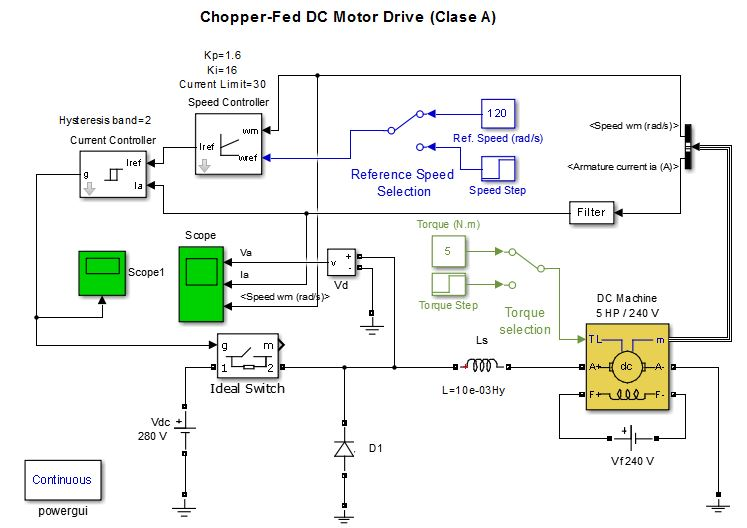
\includegraphics[scale=0.8]{imagenes/circuito.jpg}
 \caption{Circuito implementado en la simulación para el control de un motor DC}
 \label{fig:circuito}
\end{figure}

Para variar la velocidad del motor, se controla el paso de la corriente al motor a través del switch ideal, es decir se abre o cierra el circuito. Para que estas discontinuidades abruptas no generen oscilaciones en la velocidad del motor, se suavizan los cortes de corriente colocando un inductor en serie, lo que por otro lado, produce altos picos de tensión en sus extremos, por lo tanto se colocó como protección un diodo con el ánodo a masa y el cátodo entre el switch y el inductor.\\
El control se realiza a partir de la velocidad y corriente de histéresis del motor. Se realiza el calculo de la corriente que debería circular por el motor (corriente de referencia) con un controlador PI (proporcional integrador) conociendo la diferencia de velocidad que tiene el motor y la velocidad de referencia , es decir que debería tener, luego se compara dicha corriente de referencia con la corriente de histéresis del motor. Finalemente, la salida de ese comparador se utiliza para controlar el switch.\\
En la figura \ref{fig:circuito} se puede ver además, la posibilidad de usar dos controles de velocidad, una constante de $120\;rad/s$ y un escalón de velocidad que pasa de $120\;rad/s$ a $160\;rad/s$ en $t=1\;s$; y dos cargas de diferente torque en el motor una fija de $5\;N.m$ y un escalón que pasa de $5\;N.m$ a $25\;N.m$ en $t=1.5\;s$.\\

La ecuación  para calcular el torque de un motor es como sigue

\begin{equation}
T_d=T_L+B\;\omega+J\;\frac{d\omega}{dt}
\label{eq:par}
\end{equation}

Donde $T_d$ es el torque en $Nm$, $J$ el momento de inercia en $kg/m^2$, $B$ el coeficiente de fricción del motor en $N.m.s$, $\omega$ la velocidad angular en $rad/s$ y $T_L$ el torque en la carga.\\
La ecuacion que se aplica en el controlador PI para obtener la corriente de referencia es la siguiente

\begin{equation}
\frac{Out}{In}=\frac{K_i}{s}+K_p
\end{equation}

donde $K_p$ y $K_i$ son las ganancias proporcional e integral respectivamente\\


Por otro lado, cabe recordar las siguientes definiciones:

\begin{itemize}
\item $\tau_e=\frac{L_A}{R_A}$:  Es una constante de tiempo eléctrica, y se define como la rapidez con la que aumenta la corriente del motor al aplicarle un escalón de tension como entrada y manteniendo la velocidad constante. Se toman como dato la resistencia e inductancia de la armadura para calcular su valor.
\item $\tau_m=\frac{J_{T_{rem}}}{B}$: Es una constante de tiempo mecánica, y se define como la rapidez con la que el motor aumenta su velocidad angular ante un escalón de tensión como entrada, despreciando $\tau_e$ y permitiendo un cambio instantáneo de corriente. Se calcula con el momento total de inercia del motor y el coeficiente de rozamiento.
\end{itemize}

\section{Simulación}
En la figura \ref{fig:sim_cons} se ve lo que midió el osciloscopio durante la simulación con un par y velocidad fijos en $5\;Nm$ y $120\;rad/s$, y con $K_p=1,6$ y $K_i=16$ en el controlador PI.

\begin{figure}[H]
 \centering
 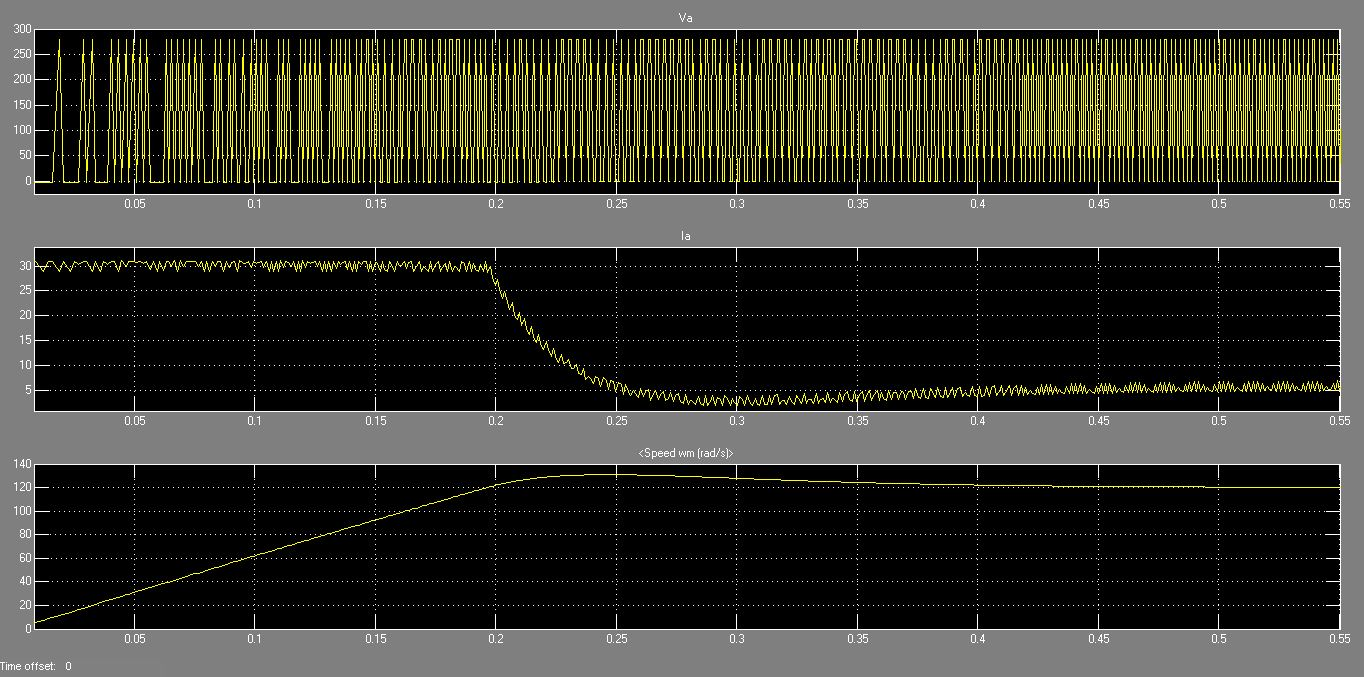
\includegraphics[scale=0.4]{imagenes/sim_cons.jpg}
 \caption{Voltaje, corriente y velocidad del motor para torque y velocidad fijos}
 \label{fig:sim_cons}
\end{figure}

Para medir la constante de tiempo eléctrica, se aplica un escalón de tensión en $t=0$, y se debe aumentar el coeficiente de rozamiento viscoso, con el objetivo de mantener constante la velocidad angular del motor. De esta forma, tenemos un sistema de primer orden y se busca el punto donde la corriente alcanza una variación del $63,2\%$ entre su valor inicial y su valor en régimen permanente.\\
En la figura \ref{fig:sim_cons_i} se ve la corriente medida por el osciloscopio.

\begin{figure}[H]
 \centering
 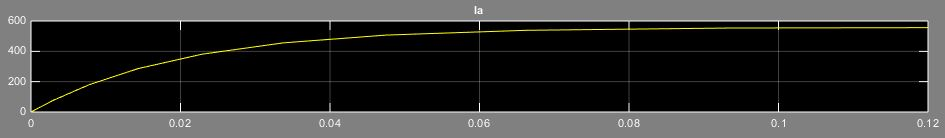
\includegraphics[scale=0.6]{imagenes/ia_cons_tau_e.jpg}
 \caption{Corriente del motor para medición de constante eléctrica}
 \label{fig:sim_cons_i}
\end{figure}

Se observa que el $63,2\%$ de la variación de la corriente desde su estado inicial hasta llegar al régimen permanente es a los $332\;A$, y el tiempo requerido fue de $0.016\;s$, que es bastante cercano al calculado: $\tau_e=\frac{0.01\;L}{0.5\;R}=0.02\;s$.\\\\


Para medir la constante de tiempo mecánica, se aumenta significativamente la resistencia de armadura, se anula la tensión de entrada y se busca el punto donde se alcance una variacion del $63,2\%$ entre el valor inicial y el de régimen. En la figura \ref{fig:sim_cons_w} se puede observar la velocidad del motor medida por el osciloscopio con las condiciones simuladas para la determinación de la constante mecánica.

\begin{figure}[H]
 \centering
 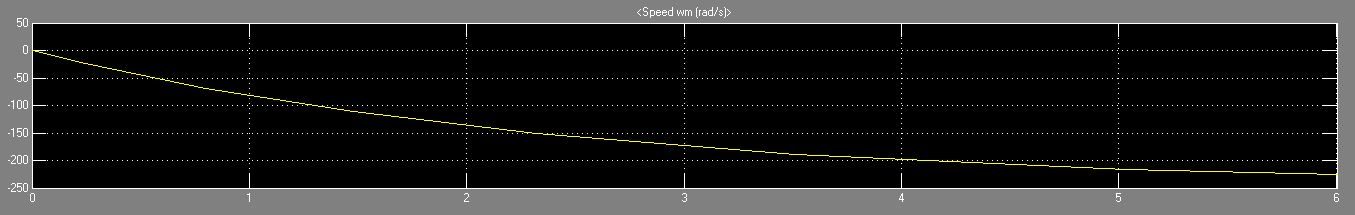
\includegraphics[scale=0.4]{imagenes/w_cons_tau_m.jpg}
 \caption{Velocidad angular del motor para medición de constante mecánica}
 \label{fig:sim_cons_w}
\end{figure}

Se puede observar que el $63,2\%$ de variacion corresponde a $151\;rad/s$, de donde se obtiene un $\tau_m$ de $2,32\;s$, que es similar al calculado de $2,5\;s$.\\\\


En la figura \ref{fig:sim_step} observa la tensión, corriente y velocidad angular del motor ante los escalones de velocidad y torque, para $K_p=1,6$ y $K_i=16$.

\begin{figure}[H]
 \centering
 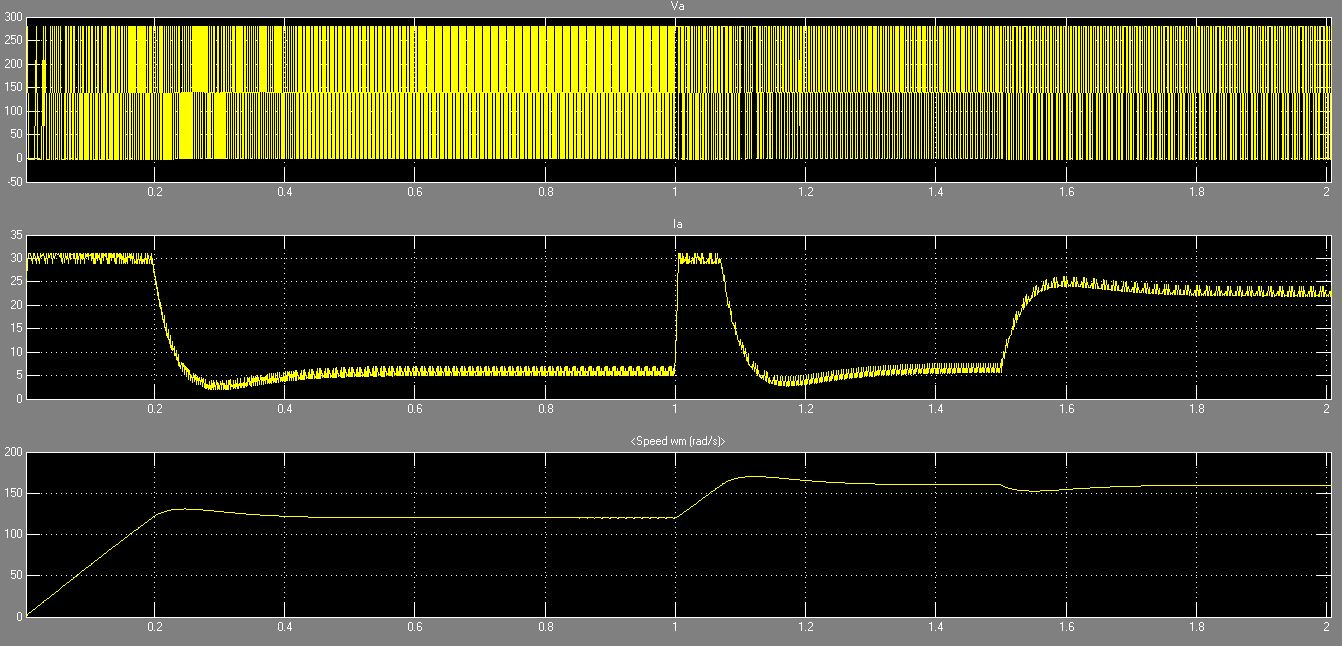
\includegraphics[scale=0.4]{imagenes/sim_step.jpg}
 \caption{Voltaje, corriente y velocidad del motor para escalones de velocidad y torque}
 \label{fig:sim_step}
\end{figure}

Se optimizaron los parámetros del controlador PI, colocando $K_p=10$ y $K_i=20$, y la respuesta del sistema con estos cambios se puede observar en la figura \ref{fig:sim_step_optimizado}

\begin{figure}[H]
 \centering
 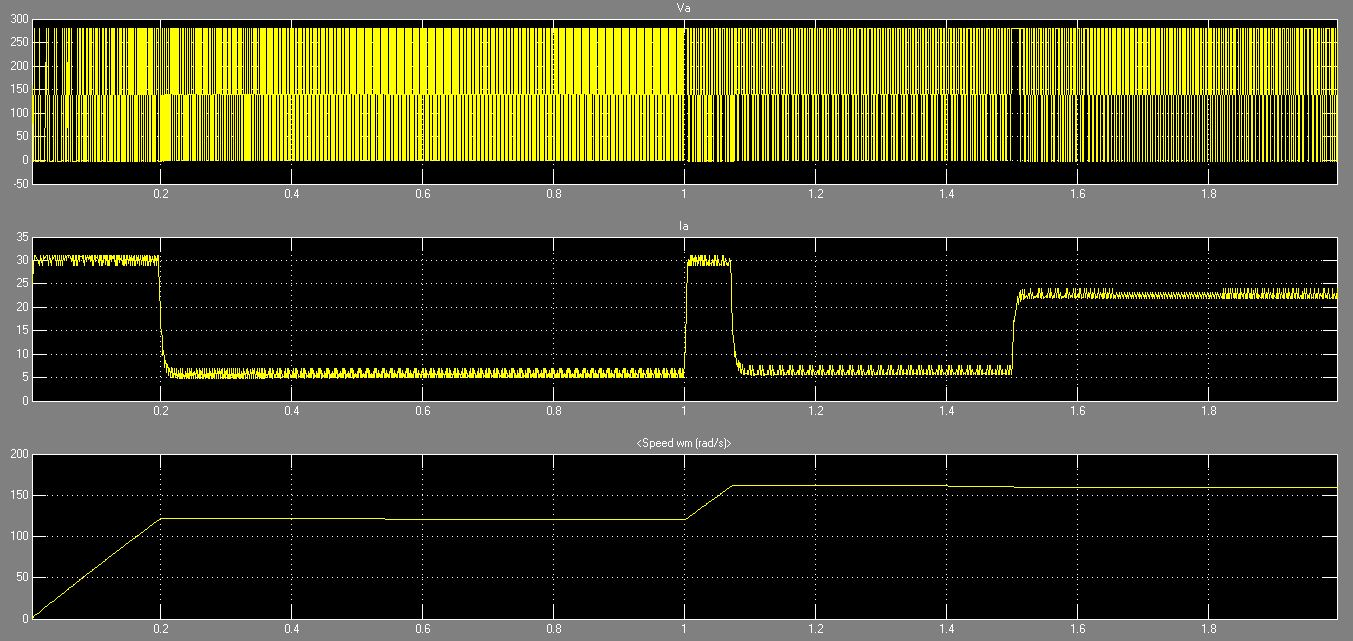
\includegraphics[scale=0.4]{imagenes/sim_step_optimizado.jpg}
 \caption{Voltaje, corriente y velocidad del motor para escalones de velocidad y torque, con controlador PI optimizado}
 \label{fig:sim_step_optimizado}
\end{figure}


Por último, en la figura \ref{fig:sim_step_limite}, se observa la respuesta del sistema con los parámetros del controlador PI originales, pero con una corriente de hasta $50\;A$

\begin{figure}[H]
 \centering
 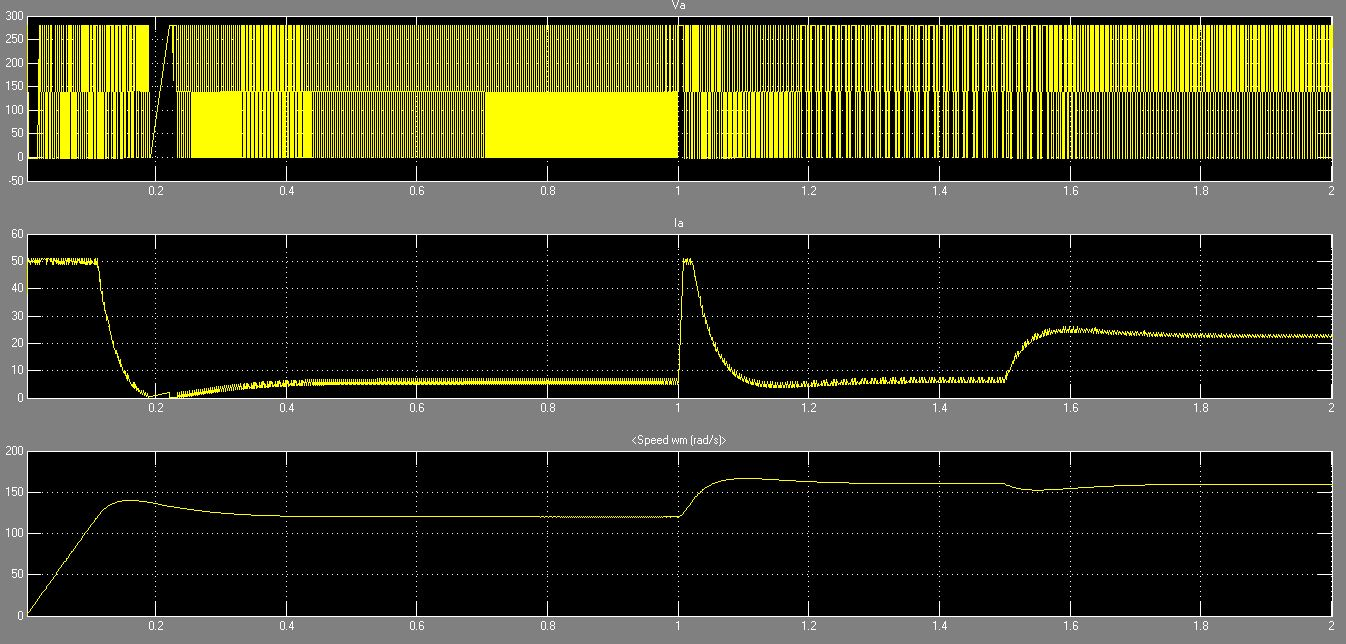
\includegraphics[scale=0.4]{imagenes/sim_step_limite.jpg}
 \caption{Voltaje, corriente y velocidad del motor para escalones de velocidad y torque, con corriente de hasta $50\;A$}
 \label{fig:sim_step_limite}
\end{figure}

\clearpage

\section{Conclusiones} 

Las constantes de tiempo eléctrica y mecánica dependen de las características físicas propias del sistema, como resistencia e inductancia de la armadura del motor, o la constante de rozamiento viscoso y el momento de inercia. Al establecer las condiciones de medición, se obtuvieron valores similares a los esperados en el cálculo teórico.\\
El par en el motor es directamente proporcional a la corriente que circula por el motor, por lo que podemos apreciar su forma al observar la corriente. Según la ecuación de torque:
\begin{center}
$T_d=T_L+B\;\omega+J\;\frac{d\omega}{dt}$
\end{center}
tanto la carga como la velocidad angular aumentan el par total en el motor; mientras que el termino que depende de la aceleración angular contribuye a los sobrepicos de corriente, en el momento de aumentar la velocidad meidante el escalón.\\
La optimización de los parámetros de un control PI es un proceso que requiere un análisis de las partes que componen el sistema y la respuesta del mismo a las distintas excitaciones. Sin embargo, variar mediante prueba y error los parámetros del filtro permitió mejorar notablemente los tiempos de establecimiento y los sobrepicos de corriente en el sistema controlado.

Al cambiar el límite de corriente, los pulsos son de menor duración pero obviamente de mayor intensidad. Esto puede utilizarse para variar los parámetros máximos de potencia admitidos por los componentes del diseño, pero no se observaron mejorías notables en la respuesta del motor al modificar dicho límite.

\section{Bibliogafía}
\begin{itemize}
\item Consigna, clases teóricas y trabajos prácticos de referencia brindados por la cátedra
\item Design and simulation of different controllers for speed control of chopper fed DC motor, Jyoti Prakash Rana, Suman Jain, Department of Electrical Engineering National Institute of Technology Rourkela
\end{itemize}


\end{document}
